\documentclass[preprint]{sigplanconf}

%% ODER: format ==         = "\mathrel{==}"
%% ODER: format /=         = "\neq "
%
%
\makeatletter
\@ifundefined{lhs2tex.lhs2tex.sty.read}%
  {\@namedef{lhs2tex.lhs2tex.sty.read}{}%
   \newcommand\SkipToFmtEnd{}%
   \newcommand\EndFmtInput{}%
   \long\def\SkipToFmtEnd#1\EndFmtInput{}%
  }\SkipToFmtEnd

\newcommand\ReadOnlyOnce[1]{\@ifundefined{#1}{\@namedef{#1}{}}\SkipToFmtEnd}
\usepackage{amstext}
\usepackage{amssymb}
\usepackage{stmaryrd}
\DeclareFontFamily{OT1}{cmtex}{}
\DeclareFontShape{OT1}{cmtex}{m}{n}
  {<5><6><7><8>cmtex8
   <9>cmtex9
   <10><10.95><12><14.4><17.28><20.74><24.88>cmtex10}{}
\DeclareFontShape{OT1}{cmtex}{m}{it}
  {<-> ssub * cmtt/m/it}{}
\newcommand{\texfamily}{\fontfamily{cmtex}\selectfont}
\DeclareFontShape{OT1}{cmtt}{bx}{n}
  {<5><6><7><8>cmtt8
   <9>cmbtt9
   <10><10.95><12><14.4><17.28><20.74><24.88>cmbtt10}{}
\DeclareFontShape{OT1}{cmtex}{bx}{n}
  {<-> ssub * cmtt/bx/n}{}
\newcommand{\tex}[1]{\text{\texfamily#1}}	% NEU

\newcommand{\Sp}{\hskip.33334em\relax}


\newcommand{\Conid}[1]{\mathit{#1}}
\newcommand{\Varid}[1]{\mathit{#1}}
\newcommand{\anonymous}{\kern0.06em \vbox{\hrule\@width.5em}}
\newcommand{\plus}{\mathbin{+\!\!\!+}}
\newcommand{\bind}{\mathbin{>\!\!\!>\mkern-6.7mu=}}
\newcommand{\rbind}{\mathbin{=\mkern-6.7mu<\!\!\!<}}% suggested by Neil Mitchell
\newcommand{\sequ}{\mathbin{>\!\!\!>}}
\renewcommand{\leq}{\leqslant}
\renewcommand{\geq}{\geqslant}
\usepackage{polytable}

%mathindent has to be defined
\@ifundefined{mathindent}%
  {\newdimen\mathindent\mathindent\leftmargini}%
  {}%

\def\resethooks{%
  \global\let\SaveRestoreHook\empty
  \global\let\ColumnHook\empty}
\newcommand*{\savecolumns}[1][default]%
  {\g@addto@macro\SaveRestoreHook{\savecolumns[#1]}}
\newcommand*{\restorecolumns}[1][default]%
  {\g@addto@macro\SaveRestoreHook{\restorecolumns[#1]}}
\newcommand*{\aligncolumn}[2]%
  {\g@addto@macro\ColumnHook{\column{#1}{#2}}}

\resethooks

\newcommand{\onelinecommentchars}{\quad-{}- }
\newcommand{\commentbeginchars}{\enskip\{-}
\newcommand{\commentendchars}{-\}\enskip}

\newcommand{\visiblecomments}{%
  \let\onelinecomment=\onelinecommentchars
  \let\commentbegin=\commentbeginchars
  \let\commentend=\commentendchars}

\newcommand{\invisiblecomments}{%
  \let\onelinecomment=\empty
  \let\commentbegin=\empty
  \let\commentend=\empty}

\visiblecomments

\newlength{\blanklineskip}
\setlength{\blanklineskip}{0.66084ex}

\newcommand{\hsindent}[1]{\quad}% default is fixed indentation
\let\hspre\empty
\let\hspost\empty
\newcommand{\NB}{\textbf{NB}}
\newcommand{\Todo}[1]{$\langle$\textbf{To do:}~#1$\rangle$}

\EndFmtInput
\makeatother
%
%
%
%
%
%
% This package provides two environments suitable to take the place
% of hscode, called "plainhscode" and "arrayhscode". 
%
% The plain environment surrounds each code block by vertical space,
% and it uses \abovedisplayskip and \belowdisplayskip to get spacing
% similar to formulas. Note that if these dimensions are changed,
% the spacing around displayed math formulas changes as well.
% All code is indented using \leftskip.
%
% Changed 19.08.2004 to reflect changes in colorcode. Should work with
% CodeGroup.sty.
%
\ReadOnlyOnce{polycode.fmt}%
\makeatletter

\newcommand{\hsnewpar}[1]%
  {{\parskip=0pt\parindent=0pt\par\vskip #1\noindent}}

% can be used, for instance, to redefine the code size, by setting the
% command to \small or something alike
\newcommand{\hscodestyle}{}

% The command \sethscode can be used to switch the code formatting
% behaviour by mapping the hscode environment in the subst directive
% to a new LaTeX environment.

\newcommand{\sethscode}[1]%
  {\expandafter\let\expandafter\hscode\csname #1\endcsname
   \expandafter\let\expandafter\endhscode\csname end#1\endcsname}

% "compatibility" mode restores the non-polycode.fmt layout.

\newenvironment{compathscode}%
  {\par\noindent
   \advance\leftskip\mathindent
   \hscodestyle
   \let\\=\@normalcr
   \let\hspre\(\let\hspost\)%
   \pboxed}%
  {\endpboxed\)%
   \par\noindent
   \ignorespacesafterend}

\newcommand{\compaths}{\sethscode{compathscode}}

% "plain" mode is the proposed default.
% It should now work with \centering.
% This required some changes. The old version
% is still available for reference as oldplainhscode.

\newenvironment{plainhscode}%
  {\hsnewpar\abovedisplayskip
   \advance\leftskip\mathindent
   \hscodestyle
   \let\hspre\(\let\hspost\)%
   \pboxed}%
  {\endpboxed%
   \hsnewpar\belowdisplayskip
   \ignorespacesafterend}

\newenvironment{oldplainhscode}%
  {\hsnewpar\abovedisplayskip
   \advance\leftskip\mathindent
   \hscodestyle
   \let\\=\@normalcr
   \(\pboxed}%
  {\endpboxed\)%
   \hsnewpar\belowdisplayskip
   \ignorespacesafterend}

% Here, we make plainhscode the default environment.

\newcommand{\plainhs}{\sethscode{plainhscode}}
\newcommand{\oldplainhs}{\sethscode{oldplainhscode}}
\plainhs

% The arrayhscode is like plain, but makes use of polytable's
% parray environment which disallows page breaks in code blocks.

\newenvironment{arrayhscode}%
  {\hsnewpar\abovedisplayskip
   \advance\leftskip\mathindent
   \hscodestyle
   \let\\=\@normalcr
   \(\parray}%
  {\endparray\)%
   \hsnewpar\belowdisplayskip
   \ignorespacesafterend}

\newcommand{\arrayhs}{\sethscode{arrayhscode}}

% The mathhscode environment also makes use of polytable's parray 
% environment. It is supposed to be used only inside math mode 
% (I used it to typeset the type rules in my thesis).

\newenvironment{mathhscode}%
  {\parray}{\endparray}

\newcommand{\mathhs}{\sethscode{mathhscode}}

% texths is similar to mathhs, but works in text mode.

\newenvironment{texthscode}%
  {\(\parray}{\endparray\)}

\newcommand{\texths}{\sethscode{texthscode}}

% The framed environment places code in a framed box.

\def\codeframewidth{\arrayrulewidth}
\RequirePackage{calc}

\newenvironment{framedhscode}%
  {\parskip=\abovedisplayskip\par\noindent
   \hscodestyle
   \arrayrulewidth=\codeframewidth
   \tabular{@{}|p{\linewidth-2\arraycolsep-2\arrayrulewidth-2pt}|@{}}%
   \hline\framedhslinecorrect\\{-1.5ex}%
   \let\endoflinesave=\\
   \let\\=\@normalcr
   \(\pboxed}%
  {\endpboxed\)%
   \framedhslinecorrect\endoflinesave{.5ex}\hline
   \endtabular
   \parskip=\belowdisplayskip\par\noindent
   \ignorespacesafterend}

\newcommand{\framedhslinecorrect}[2]%
  {#1[#2]}

\newcommand{\framedhs}{\sethscode{framedhscode}}

% The inlinehscode environment is an experimental environment
% that can be used to typeset displayed code inline.

\newenvironment{inlinehscode}%
  {\(\def\column##1##2{}%
   \let\>\undefined\let\<\undefined\let\\\undefined
   \newcommand\>[1][]{}\newcommand\<[1][]{}\newcommand\\[1][]{}%
   \def\fromto##1##2##3{##3}%
   \def\nextline{}}{\) }%

\newcommand{\inlinehs}{\sethscode{inlinehscode}}

% The joincode environment is a separate environment that
% can be used to surround and thereby connect multiple code
% blocks.

\newenvironment{joincode}%
  {\let\orighscode=\hscode
   \let\origendhscode=\endhscode
   \def\endhscode{\def\hscode{\endgroup\def\@currenvir{hscode}\\}\begingroup}
   %\let\SaveRestoreHook=\empty
   %\let\ColumnHook=\empty
   %\let\resethooks=\empty
   \orighscode\def\hscode{\endgroup\def\@currenvir{hscode}}}%
  {\origendhscode
   \global\let\hscode=\orighscode
   \global\let\endhscode=\origendhscode}%

\makeatother
\EndFmtInput
%
%
\ReadOnlyOnce{agda.fmt}%


\RequirePackage[T1]{fontenc}
\RequirePackage[utf8x]{inputenc}
\RequirePackage{ucs}
\RequirePackage{amsfonts}

\providecommand\mathbbm{\mathbb}

% TODO: Define more of these ...
\DeclareUnicodeCharacter{737}{\textsuperscript{l}}
\DeclareUnicodeCharacter{8718}{\ensuremath{\blacksquare}}
\DeclareUnicodeCharacter{8759}{::}
\DeclareUnicodeCharacter{9669}{\ensuremath{\triangleleft}}
\DeclareUnicodeCharacter{8799}{\ensuremath{\stackrel{\scriptscriptstyle ?}{=}}}
\DeclareUnicodeCharacter{10214}{\ensuremath{\llbracket}}
\DeclareUnicodeCharacter{10215}{\ensuremath{\rrbracket}}

% TODO: This is in general not a good idea.
\providecommand\textepsilon{$\epsilon$}
\providecommand\textmu{$\mu$}


%Actually, varsyms should not occur in Agda output.

% TODO: Make this configurable. IMHO, italics doesn't work well
% for Agda code.

\renewcommand\Varid[1]{\mathord{\textsf{#1}}}
\let\Conid\Varid
\newcommand\Keyword[1]{\textsf{\textbf{#1}}}
\EndFmtInput

% Packages
\usepackage{amsmath}%
\usepackage{tikz}%
\usepackage{tikz-qtree}%
\usepackage{subfigure}%
\usetikzlibrary{arrows,positioning}%
\usepackage{listings}%
\usepackage{url}%
\usepackage{wasysym}%

% Unicode support
\usepackage{textgreek}
\usepackage{ucs}
\usepackage[utf8x]{inputenc}

\DeclareUnicodeCharacter{948}{\ensuremath{\delta}}
\DeclareUnicodeCharacter{955}{\ensuremath{\lambda}}

% Coloured comments
\usepackage{color}
\usepackage{ifthen}
\newboolean{showNotes}
\newboolean{marginNotes}
\setboolean{showNotes}{false}
\setboolean{marginNotes}{false}
\newcommand{\marginNote}[1]{
\ifthenelse
  {\boolean{marginNotes}}
  {\marginpar{#1}}
  {#1}}

\newcommand{\todo}[1]{
\ifthenelse
  {\boolean{showNotes}}
  {\marginNote{\textcolor{red}{\textbf{Todo:~}#1}}}
  {}}

\newcommand{\wouter}[1]{
\ifthenelse
  {\boolean{showNotes}}
  {\marginNote{\textcolor{blue}{\textbf{Wouter:~}#1}}}
  {}}

\newcommand{\pepijn}[1]{
\ifthenelse
  {\boolean{showNotes}}
  {\marginNote{\textcolor{blue}{\textbf{Pepijn:~}#1}}}
  {}}


\begin{document}

\conferenceinfo{CPP'15} {January 12--14, 2015, Mumbai, India}
\titlebanner{Under preparation for CPP 2015}

\title{Auto in Agda}
\subtitle{Programming proof search}

\authorinfo{Pepijn Kokke \and Wouter Swierstra}
           {Universiteit Utrecht}
           {pepijn.kokke@gmail.com \quad w.s.swierstra@uu.nl}

\maketitle

\begin{abstract}

  As proofs in type theory become increasingly complex, there is a
  growing need to provide better proof automation. This paper shows
  how to implement a Prolog-style resolution procedure in the
  dependently typed programming language Agda. Connecting this
  resolution procedure to Agda's reflection mechanism provides a
  first-class proof search tactic for first-order Agda
  terms. Furthermore, the same mechanism may be used in tandem with
  Agda's instance arguments to implement type classes in the style of
  Haskell. As a result, writing proof automation tactics need not be
  different from writing any other program.

\end{abstract}

%%include intro.lagda
%%include motivation.lagda
\section{Proof search in Agda}
\label{sec:prolog}

The following section describes our implementation of proof search
à la Prolog in Agda. This implementation abstracts over two data types
for names---one for inference rules and one for term constructors.
These data types will be referred to as \ensuremath{\Conid{RuleName}} and \ensuremath{\Conid{TermName}}, and
will be instantiated with types (with the same names) in
section~\ref{sec:reflection}.


\subsection*{Terms and unification}

The heart of our proof search implementation is the structurally
recursive unification algorithm described by~\citet{unification}. Here
the type of terms is indexed by the number of variables a given term
may contain. Doing so enables the formulation of the unification
algorithm by structural induction on the number of free variables.
For this to work, we will use the following definition of
terms\footnote{
  We will use the name \ensuremath{\Conid{PsTerm}} to stand for \emph{proof search term}
  to differentiate them from Agda's \emph{reflection terms}, or \ensuremath{\Conid{AgTerm}}.
}:
\begin{hscode}\SaveRestoreHook
\column{B}{@{}>{\hspre}l<{\hspost}@{}}%
\column{3}{@{}>{\hspre}l<{\hspost}@{}}%
\column{8}{@{}>{\hspre}l<{\hspost}@{}}%
\column{E}{@{}>{\hspre}l<{\hspost}@{}}%
\>[B]{}\Keyword{data}\;\Conid{PsTerm}\;(\Varid{n}\;\mathbin{:}\;\Conid{ℕ})\;\mathbin{:}\;\Conid{Set}\;\Keyword{where}{}\<[E]%
\\
\>[B]{}\hsindent{3}{}\<[3]%
\>[3]{}\Varid{var}\;{}\<[8]%
\>[8]{}\mathbin{:}\;\Conid{Fin}\;\Varid{n}\;\Varid{→}\;\Conid{PsTerm}\;\Varid{n}{}\<[E]%
\\
\>[B]{}\hsindent{3}{}\<[3]%
\>[3]{}\Varid{con}\;{}\<[8]%
\>[8]{}\mathbin{:}\;\Conid{TermName}\;\Varid{→}\;\Conid{List}\;(\Conid{PsTerm}\;\Varid{n})\;\Varid{→}\;\Conid{PsTerm}\;\Varid{n}{}\<[E]%
\ColumnHook
\end{hscode}\resethooks
In addition to a restricted set of variables, we will allow
first-order constants encoded as a name with a list of
arguments.

For instance, if we choose to instantiate \ensuremath{\Conid{PsName}} with the following
\ensuremath{\Conid{Arith}} data type, we can encode numbers and simple arithmetic
expressions:
\begin{hscode}\SaveRestoreHook
\column{B}{@{}>{\hspre}l<{\hspost}@{}}%
\column{3}{@{}>{\hspre}l<{\hspost}@{}}%
\column{9}{@{}>{\hspre}l<{\hspost}@{}}%
\column{E}{@{}>{\hspre}l<{\hspost}@{}}%
\>[B]{}\Keyword{data}\;\Conid{Arith}\;\mathbin{:}\;\Conid{Set}\;\Keyword{where}{}\<[E]%
\\
\>[B]{}\hsindent{3}{}\<[3]%
\>[3]{}\Conid{Suc}\;{}\<[9]%
\>[9]{}\mathbin{:}\;\Conid{Arith}{}\<[E]%
\\
\>[B]{}\hsindent{3}{}\<[3]%
\>[3]{}\Conid{Zero}\;{}\<[9]%
\>[9]{}\mathbin{:}\;\Conid{Arith}{}\<[E]%
\\
\>[B]{}\hsindent{3}{}\<[3]%
\>[3]{}\Conid{Add}\;{}\<[9]%
\>[9]{}\mathbin{:}\;\Conid{Arith}{}\<[E]%
\ColumnHook
\end{hscode}\resethooks
The closed term corresponding to the number one could be written as follows:
\begin{hscode}\SaveRestoreHook
\column{B}{@{}>{\hspre}l<{\hspost}@{}}%
\column{E}{@{}>{\hspre}l<{\hspost}@{}}%
\>[B]{}\Conid{One}\;\mathbin{:}\;\Conid{PsTerm}\;\Varid{0}{}\<[E]%
\\
\>[B]{}\Conid{One}\;\mathrel{=}\;\Varid{con}\;\Conid{Suc}\;(\Varid{con}\;\Conid{Zero}\;[\mskip1.5mu \mskip1.5mu]\;\Varid{∷}\;[\mskip1.5mu \mskip1.5mu]){}\<[E]%
\ColumnHook
\end{hscode}\resethooks
Similarly, we can use the \ensuremath{\Varid{var}} constructor to represent open terms,
such as \ensuremath{\Varid{x}\;\Varid{+}\;\Varid{1}}. We use the prefix operator \ensuremath{\Varid{\#}} to convert from
natural numbers to finite types:
\begin{hscode}\SaveRestoreHook
\column{B}{@{}>{\hspre}l<{\hspost}@{}}%
\column{E}{@{}>{\hspre}l<{\hspost}@{}}%
\>[B]{}\Conid{AddOne}\;\mathbin{:}\;\Conid{PsTerm}\;\Varid{1}{}\<[E]%
\\
\>[B]{}\Conid{AddOne}\;\mathrel{=}\;\Varid{con}\;\Conid{Add}\;(\Varid{var}\;(\Varid{\#}\;\Varid{0})\;\Varid{∷}\;\Varid{con}\;\Conid{One}\;[\mskip1.5mu \mskip1.5mu]\;\Varid{∷}\;[\mskip1.5mu \mskip1.5mu]){}\<[E]%
\ColumnHook
\end{hscode}\resethooks
Note that this representation of terms is untyped. There is no check
that enforces addition is provided precisely two arguments. Although
we could add further type information to this effect, this introduces
additional overhead without adding safety to the proof automation
presented in this paper. For the sake of simplicity, we have therefore
chosen to work with this untyped definition.

We shall refrain from further discussion of the unification algorithm itself.
Instead, we restrict ourselves to presenting the interface that we will use:
\begin{hscode}\SaveRestoreHook
\column{B}{@{}>{\hspre}l<{\hspost}@{}}%
\column{3}{@{}>{\hspre}l<{\hspost}@{}}%
\column{10}{@{}>{\hspre}l<{\hspost}@{}}%
\column{E}{@{}>{\hspre}l<{\hspost}@{}}%
\>[3]{}\Varid{unify}\;{}\<[10]%
\>[10]{}\mathbin{:}\;(\Varid{t₁}\;\Varid{t₂}\;\mathbin{:}\;\Conid{PsTerm}\;\Varid{m})\;\Varid{→}\;\Conid{Maybe}\;(\Varid{∃}\;[\mskip1.5mu \Varid{n}\mskip1.5mu]\;\Conid{Subst}\;\Varid{m}\;\Varid{n}){}\<[E]%
\ColumnHook
\end{hscode}\resethooks
The \ensuremath{\Varid{unify}} function takes two terms \ensuremath{\Varid{t₁}} and \ensuremath{\Varid{t₂}} and tries to
compute a sustitution---the most general unifier. Substitutions are
indexed by two natural numbers \ensuremath{\Varid{m}} and \ensuremath{\Varid{n}}. A substitution of type
\ensuremath{\Conid{Subst}\;\Varid{m}\;\Varid{n}} can be applied to a \ensuremath{\Conid{PsTerm}\;\Varid{m}} to produce a value of type
\ensuremath{\Conid{PsTerm}\;\Varid{n}}.
As unification may fail, the result is wrapped in the \ensuremath{\Conid{Maybe}} type. In
addition, since the number of variables in the terms resulting from
the unifying substitution is not known \emph{a priori}, this
number is existentially quantified over.
For the remainder of the paper, we will write \ensuremath{\Varid{∃}\;[\mskip1.5mu \Varid{x}\mskip1.5mu]\;\Conid{B}} to mean a
type \ensuremath{\Conid{B}} with occurrences of an existentially quantified variable \ensuremath{\Varid{x}},
or \ensuremath{\Varid{∃}\;(\Varid{λ}\;\Varid{x}\;\Varid{→}\;\Conid{B})} in full.

Occasionally we will use a more general function \ensuremath{\Varid{unifyAcc}}, which
takes a substitution as an additional parameter. It applies this
substitution to \ensuremath{\Varid{t₁}} and \ensuremath{\Varid{t₂}} before attempting to unify.
\begin{hscode}\SaveRestoreHook
\column{B}{@{}>{\hspre}l<{\hspost}@{}}%
\column{3}{@{}>{\hspre}l<{\hspost}@{}}%
\column{13}{@{}>{\hspre}l<{\hspost}@{}}%
\column{E}{@{}>{\hspre}l<{\hspost}@{}}%
\>[3]{}\Varid{unifyAcc}\;{}\<[13]%
\>[13]{}\mathbin{:}\;(\Varid{t₁}\;\Varid{t₂}\;\mathbin{:}\;\Conid{PsTerm}\;\Varid{m})\;{}\<[E]%
\\
\>[13]{}\Varid{→}\;\Varid{∃}\;[\mskip1.5mu \Varid{n}\mskip1.5mu]\;\Conid{Subst}\;\Varid{m}\;\Varid{n}\;\Varid{→}\;\Conid{Maybe}\;(\Varid{∃}\;[\mskip1.5mu \Varid{n}\mskip1.5mu]\;\Conid{Subst}\;\Varid{m}\;\Varid{n}){}\<[E]%
\ColumnHook
\end{hscode}\resethooks


\subsection*{Inference rules}

We encode inference rules as records containing a rule name, a list of
terms for its premises, and a term for its conclusion:
\begin{hscode}\SaveRestoreHook
\column{B}{@{}>{\hspre}l<{\hspost}@{}}%
\column{3}{@{}>{\hspre}l<{\hspost}@{}}%
\column{5}{@{}>{\hspre}l<{\hspost}@{}}%
\column{7}{@{}>{\hspre}l<{\hspost}@{}}%
\column{19}{@{}>{\hspre}l<{\hspost}@{}}%
\column{E}{@{}>{\hspre}l<{\hspost}@{}}%
\>[3]{}\Keyword{record}\;\Conid{Rule}\;(\Varid{n}\;\mathbin{:}\;\Conid{ℕ})\;\mathbin{:}\;\Conid{Set}\;\Keyword{where}{}\<[E]%
\\
\>[3]{}\hsindent{2}{}\<[5]%
\>[5]{}\Keyword{field}{}\<[E]%
\\
\>[5]{}\hsindent{2}{}\<[7]%
\>[7]{}\Varid{name}\;{}\<[19]%
\>[19]{}\mathbin{:}\;\Conid{RuleName}{}\<[E]%
\\
\>[5]{}\hsindent{2}{}\<[7]%
\>[7]{}\Varid{premises}\;{}\<[19]%
\>[19]{}\mathbin{:}\;\Conid{List}\;(\Conid{PsTerm}\;\Varid{n}){}\<[E]%
\\
\>[5]{}\hsindent{2}{}\<[7]%
\>[7]{}\Varid{conclusion}\;{}\<[19]%
\>[19]{}\mathbin{:}\;\Conid{PsTerm}\;\Varid{n}{}\<[E]%
\ColumnHook
\end{hscode}\resethooks
Once again the data-type is quantified over the number of variables
used in the rule. Note that the variables are shared between the
premises and the conclusion.

Using our newly defined \ensuremath{\Conid{Rule}} we can give a simple definition of
addition. In Prolog, this would be written as follows.
\begin{tabbing}\tt
~~~add\char40{}0\char44{}~X\char44{}~X\char41{}\char46{}\\
\tt ~~~add\char40{}suc\char40{}X\char41{}\char44{}~Y\char44{}~suc\char40{}Z\char41{}\char41{}~\char58{}\char45{}~add\char40{}X\char44{}~Y\char44{}~Z\char41{}\char46{}
\end{tabbing}
Unfortunately, the named equivalents in our Agda implementation are a
bit more verbose. Note that we have, for the sake of this example,
instantiated the \ensuremath{\Conid{RuleName}} and \ensuremath{\Conid{TermName}} to \ensuremath{\Conid{String}} and \ensuremath{\Conid{Arith}}
respectively.
\begin{hscode}\SaveRestoreHook
\column{B}{@{}>{\hspre}l<{\hspost}@{}}%
\column{3}{@{}>{\hspre}l<{\hspost}@{}}%
\column{15}{@{}>{\hspre}l<{\hspost}@{}}%
\column{26}{@{}>{\hspre}l<{\hspost}@{}}%
\column{29}{@{}>{\hspre}l<{\hspost}@{}}%
\column{E}{@{}>{\hspre}l<{\hspost}@{}}%
\>[B]{}\Conid{AddBase}\;\mathbin{:}\;\Conid{Rule}\;\Varid{1}{}\<[E]%
\\
\>[B]{}\Conid{AddBase}\;\mathrel{=}\;\Keyword{record}\;\{\mskip1.5mu {}\<[E]%
\\
\>[B]{}\hsindent{3}{}\<[3]%
\>[3]{}\Varid{name}\;{}\<[15]%
\>[15]{}\mathrel{=}\;\text{\tt \char34 AddBase\char34}{}\<[E]%
\\
\>[B]{}\hsindent{3}{}\<[3]%
\>[3]{}\Varid{conclusion}\;{}\<[15]%
\>[15]{}\mathrel{=}\;\Varid{con}\;\Conid{Add}\;{}\<[26]%
\>[26]{}({}\<[29]%
\>[29]{}\Varid{con}\;\Conid{Zero}\;[\mskip1.5mu \mskip1.5mu]{}\<[E]%
\\
\>[26]{}\Varid{∷}\;{}\<[29]%
\>[29]{}\Varid{var}\;(\Varid{\#}\;\Varid{0}){}\<[E]%
\\
\>[26]{}\Varid{∷}\;{}\<[29]%
\>[29]{}\Varid{var}\;(\Varid{\#}\;\Varid{0}){}\<[E]%
\\
\>[26]{}\Varid{∷}\;[\mskip1.5mu \mskip1.5mu]){}\<[E]%
\\
\>[B]{}\hsindent{3}{}\<[3]%
\>[3]{}\Varid{premises}\;{}\<[15]%
\>[15]{}\mathrel{=}\;[\mskip1.5mu \mskip1.5mu]{}\<[E]%
\\
\>[B]{}\hsindent{3}{}\<[3]%
\>[3]{}\mskip1.5mu\}{}\<[E]%
\ColumnHook
\end{hscode}\resethooks
%
\begin{hscode}\SaveRestoreHook
\column{B}{@{}>{\hspre}l<{\hspost}@{}}%
\column{3}{@{}>{\hspre}l<{\hspost}@{}}%
\column{15}{@{}>{\hspre}l<{\hspost}@{}}%
\column{18}{@{}>{\hspre}l<{\hspost}@{}}%
\column{27}{@{}>{\hspre}l<{\hspost}@{}}%
\column{30}{@{}>{\hspre}l<{\hspost}@{}}%
\column{E}{@{}>{\hspre}l<{\hspost}@{}}%
\>[B]{}\Conid{AddStep}\;\mathbin{:}\;\Conid{Rule}\;\Varid{3}{}\<[E]%
\\
\>[B]{}\Conid{AddStep}\;\mathrel{=}\;\Keyword{record}\;\{\mskip1.5mu {}\<[E]%
\\
\>[B]{}\hsindent{3}{}\<[3]%
\>[3]{}\Varid{name}\;{}\<[15]%
\>[15]{}\mathrel{=}\;\text{\tt \char34 AddStep\char34}{}\<[E]%
\\
\>[B]{}\hsindent{3}{}\<[3]%
\>[3]{}\Varid{conclusion}\;{}\<[15]%
\>[15]{}\mathrel{=}\;{}\<[18]%
\>[18]{}\Varid{con}\;\Conid{Add}\;{}\<[27]%
\>[27]{}({}\<[30]%
\>[30]{}\Varid{con}\;\Conid{Suc}\;(\Varid{var}\;(\Varid{\#}\;\Varid{0})\;\Varid{∷}\;[\mskip1.5mu \mskip1.5mu]){}\<[E]%
\\
\>[27]{}\Varid{∷}\;{}\<[30]%
\>[30]{}\Varid{var}\;(\Varid{\#}\;\Varid{1}){}\<[E]%
\\
\>[27]{}\Varid{∷}\;{}\<[30]%
\>[30]{}\Varid{con}\;\Conid{Suc}\;(\Varid{var}\;(\Varid{\#}\;\Varid{2})\;\Varid{∷}\;[\mskip1.5mu \mskip1.5mu]){}\<[E]%
\\
\>[27]{}\Varid{∷}\;[\mskip1.5mu \mskip1.5mu]){}\<[E]%
\\
\>[B]{}\hsindent{3}{}\<[3]%
\>[3]{}\Varid{premises}\;{}\<[15]%
\>[15]{}\mathrel{=}\;{}\<[18]%
\>[18]{}\Varid{con}\;\Conid{Add}\;{}\<[27]%
\>[27]{}({}\<[30]%
\>[30]{}\Varid{var}\;(\Varid{\#}\;\Varid{0}){}\<[E]%
\\
\>[27]{}\Varid{∷}\;{}\<[30]%
\>[30]{}\Varid{var}\;(\Varid{\#}\;\Varid{1}){}\<[E]%
\\
\>[27]{}\Varid{∷}\;{}\<[30]%
\>[30]{}\Varid{var}\;(\Varid{\#}\;\Varid{2}){}\<[E]%
\\
\>[27]{}\Varid{∷}\;[\mskip1.5mu \mskip1.5mu])\;{}\<[E]%
\\
\>[18]{}\Varid{∷}\;[\mskip1.5mu \mskip1.5mu]{}\<[E]%
\\
\>[B]{}\hsindent{3}{}\<[3]%
\>[3]{}\mskip1.5mu\}{}\<[E]%
\ColumnHook
\end{hscode}\resethooks


\subsection*{Generalised injection and raising}

Before we can implement some form of proof search, we define a pair of
auxiliary functions. During proof resolution, we will need to work
with terms and rules containing a different number of variables. We
will use the following pair of functions, \ensuremath{\Varid{inject}} and \ensuremath{\Varid{raise}}, to
weaken bound variables, that is, map values of type \ensuremath{\Conid{Fin}\;\Varid{n}} to some
larger finite type.
\begin{hscode}\SaveRestoreHook
\column{B}{@{}>{\hspre}l<{\hspost}@{}}%
\column{3}{@{}>{\hspre}l<{\hspost}@{}}%
\column{10}{@{}>{\hspre}l<{\hspost}@{}}%
\column{13}{@{}>{\hspre}l<{\hspost}@{}}%
\column{18}{@{}>{\hspre}l<{\hspost}@{}}%
\column{21}{@{}>{\hspre}l<{\hspost}@{}}%
\column{E}{@{}>{\hspre}l<{\hspost}@{}}%
\>[3]{}\Varid{inject}\;\mathbin{:}\;\Varid{∀}\;\{\mskip1.5mu \Varid{m}\mskip1.5mu\}\;\Varid{n}\;\Varid{→}\;\Conid{Fin}\;\Varid{m}\;\Varid{→}\;\Conid{Fin}\;(\Varid{m}\;\Varid{+}\;\Varid{n}){}\<[E]%
\\
\>[3]{}\Varid{inject}\;\Varid{n}\;{}\<[13]%
\>[13]{}\Varid{zero}\;{}\<[21]%
\>[21]{}\mathrel{=}\;\Varid{zero}{}\<[E]%
\\
\>[3]{}\Varid{inject}\;\Varid{n}\;(\Varid{suc}\;\Varid{i})\;{}\<[21]%
\>[21]{}\mathrel{=}\;\Varid{suc}\;(\Varid{inject}\;\Varid{n}\;\Varid{i}){}\<[E]%
\\[\blanklineskip]%
\>[3]{}\Varid{raise}\;\mathbin{:}\;\Varid{∀}\;\Varid{m}\;\{\mskip1.5mu \Varid{n}\mskip1.5mu\}\;\Varid{→}\;\Conid{Fin}\;\Varid{n}\;\Varid{→}\;\Conid{Fin}\;(\Varid{m}\;\Varid{+}\;\Varid{n}){}\<[E]%
\\
\>[3]{}\Varid{raise}\;{}\<[10]%
\>[10]{}\Varid{zero}\;{}\<[18]%
\>[18]{}\Varid{i}\;{}\<[21]%
\>[21]{}\mathrel{=}\;\Varid{i}{}\<[E]%
\\
\>[3]{}\Varid{raise}\;(\Varid{suc}\;\Varid{m})\;{}\<[18]%
\>[18]{}\Varid{i}\;{}\<[21]%
\>[21]{}\mathrel{=}\;\Varid{suc}\;(\Varid{raise}\;\Varid{m}\;\Varid{i}){}\<[E]%
\ColumnHook
\end{hscode}\resethooks
We have tried to visualize the behaviour of \ensuremath{\Varid{inject}} and \ensuremath{\Varid{raise}},
embedding \ensuremath{\Conid{Fin}\;\Varid{3}} into \ensuremath{\Conid{Fin}\;(\Varid{3}\;\Varid{+}\;\Varid{1})} in Figure~\ref{fig:fins}. On the
surface, the \ensuremath{\Varid{inject}} function appears to be the identity. When you
make all the implicit arguments explicit, however, you will see that
it sends the \ensuremath{\Varid{zero}} constructor in \ensuremath{\Conid{Fin}\;\Varid{m}} to the \ensuremath{\Varid{zero}} constructor
of type \ensuremath{\Conid{Fin}\;(\Varid{m}\;\Varid{+}\;\Varid{n})}. Hence, the \ensuremath{\Varid{inject}} function maps \ensuremath{\Conid{Fin}\;\Varid{m}} into the
\emph{first} \ensuremath{\Varid{m}} elements of the type \ensuremath{\Conid{Fin}\;(\Varid{m}\;\Varid{+}\;\Varid{n})}. Dually, the
\ensuremath{\Varid{raise}} function maps \ensuremath{\Conid{Fin}\;\Varid{n}} into the \emph{last} \ensuremath{\Varid{n}} elements of the
type \ensuremath{\Conid{Fin}\;(\Varid{m}\;\Varid{+}\;\Varid{n})} by repeatedly applying the \ensuremath{\Varid{suc}} constructor.

\begin{figure}
  \centering
  \subfigure[]{ \label{fig:injFig}
    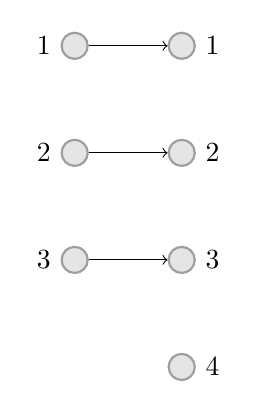
\begin{tikzpicture}[place/.style={circle,draw=darkgray!50,fill=gray!20,thick}]
       \node[place,label=left:1] (one3) {};
       \node[place,label=left:2] (two3) [below=of one3] {};
       \node[place,label=left:3] (three3) [below=of two3] {};

       \node[place,label=right:1] (one4) [right=of one3] {};
       \node[place,label=right:2] (two4) [below=of one4] {};
       \node[place,label=right:3] (three4) [below=of two4] {};
       \node[place,label=right:4] (four4) [below=of three4] {};

       \draw [->] (one3) to [thick, shorten <=1pt,>=stealth'] (one4);
       \draw [->] (two3) to [thick, shorten <=1pt,>=stealth']  (two4);
       \draw [->] (three3) to [thick, shorten <=1pt,>=stealth']  (three4);
    \end{tikzpicture}}
\hspace{7.5em}
  \subfigure[]{
  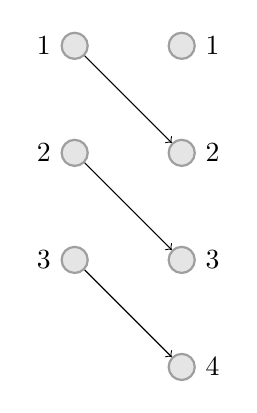
\begin{tikzpicture} [place/.style={circle,draw=darkgray!50,fill=gray!20,thick}]
       \node[place,label=left:1] (one3) {};
       \node[place,label=left:2] (two3) [below=of one3] {};
       \node[place,label=left:3] (three3) [below=of two3] {};

       \node[place,label=right:1] (one4) [right=of one3] {};
       \node[place,label=right:2] (two4) [below=of one4] {};
       \node[place,label=right:3] (three4) [below=of two4] {};
       \node[place,label=right:4] (four4) [below=of three4] {};

       \draw [->] (one3) to [thick, shorten <=1pt,>=stealth'] (two4);
       \draw [->] (two3) to [thick, shorten <=1pt,>=stealth']  (three4);
       \draw [->] (three3) to [thick, shorten <=1pt,>=stealth']  (four4);
  \end{tikzpicture}}

\vspace{4ex}
\caption{The graph of the \ensuremath{\Varid{inject}} function (a) and the \ensuremath{\Varid{raise}}
  function (b) embedding \ensuremath{\Conid{Fin}\;\Varid{3}} in \ensuremath{\Conid{Fin}\;(\Varid{3}\;\Varid{+}\;\Varid{1})}}
  \label{fig:fins}
\end{figure}
We can use these \ensuremath{\Varid{inject}} and \ensuremath{\Varid{raise}} to define similar functions
that work on our \ensuremath{\Conid{Rule}} and \ensuremath{\Conid{Term}} data types, by mapping them over
all the variables that they contain.


\subsection*{Constructing the search tree}

\begin{hscode}\SaveRestoreHook
\column{B}{@{}>{\hspre}l<{\hspost}@{}}%
\column{3}{@{}>{\hspre}l<{\hspost}@{}}%
\column{5}{@{}>{\hspre}l<{\hspost}@{}}%
\column{E}{@{}>{\hspre}l<{\hspost}@{}}%
\>[3]{}\Keyword{data}\;\Conid{SearchTree}\;(\Conid{A}\;\mathbin{:}\;\Conid{Set})\;\mathbin{:}\;\Conid{Set}\;\Keyword{where}{}\<[E]%
\\
\>[3]{}\hsindent{2}{}\<[5]%
\>[5]{}\Varid{fail}\;\mathbin{:}\;\Conid{SearchTree}\;\Conid{A}{}\<[E]%
\\
\>[3]{}\hsindent{2}{}\<[5]%
\>[5]{}\Varid{retn}\;\mathbin{:}\;\Conid{A}\;\Varid{→}\;\Conid{SearchTree}\;\Conid{A}{}\<[E]%
\\
\>[3]{}\hsindent{2}{}\<[5]%
\>[5]{}\Varid{fork}\;\mathbin{:}\;\Conid{List}\;(\Varid{∞}\;(\Conid{SearchTree}\;\Conid{A}))\;\Varid{→}\;\Conid{SearchTree}\;\Conid{A}{}\<[E]%
\ColumnHook
\end{hscode}\resethooks

\begin{hscode}\SaveRestoreHook
\column{B}{@{}>{\hspre}l<{\hspost}@{}}%
\column{3}{@{}>{\hspre}l<{\hspost}@{}}%
\column{5}{@{}>{\hspre}l<{\hspost}@{}}%
\column{E}{@{}>{\hspre}l<{\hspost}@{}}%
\>[3]{}\Keyword{data}\;\Conid{Proof}\;\mathbin{:}\;\Conid{Set}\;\Keyword{where}{}\<[E]%
\\
\>[3]{}\hsindent{2}{}\<[5]%
\>[5]{}\Varid{con}\;\mathbin{:}\;(\Varid{name}\;\mathbin{:}\;\Conid{RuleName})\;(\Varid{args}\;\mathbin{:}\;\Conid{List}\;\Conid{Proof})\;\Varid{→}\;\Conid{Proof}{}\<[E]%
\ColumnHook
\end{hscode}\resethooks

\begin{hscode}\SaveRestoreHook
\column{B}{@{}>{\hspre}l<{\hspost}@{}}%
\column{3}{@{}>{\hspre}l<{\hspost}@{}}%
\column{E}{@{}>{\hspre}l<{\hspost}@{}}%
\>[3]{}\Conid{Proof′}\;\mathbin{:}\;\Conid{ℕ}\;\Varid{→}\;\Conid{Set}{}\<[E]%
\\
\>[3]{}\Conid{Proof′}\;\Varid{m}\;\mathrel{=}\;\Varid{∃}\;[\mskip1.5mu \Varid{k}\mskip1.5mu]\;\Conid{Vec}\;(\Conid{Goal}\;\Varid{m})\;\Varid{k}\;\Varid{×}\;(\Conid{Vec}\;\Conid{Proof}\;\Varid{k}\;\Varid{→}\;\Conid{Proof}){}\<[E]%
\ColumnHook
\end{hscode}\resethooks

\begin{hscode}\SaveRestoreHook
\column{B}{@{}>{\hspre}l<{\hspost}@{}}%
\column{3}{@{}>{\hspre}l<{\hspost}@{}}%
\column{5}{@{}>{\hspre}l<{\hspost}@{}}%
\column{E}{@{}>{\hspre}l<{\hspost}@{}}%
\>[3]{}\Varid{con′}\;\mathbin{:}\;{}\<[E]%
\\
\>[3]{}\hsindent{2}{}\<[5]%
\>[5]{}(\Varid{r}\;\mathbin{:}\;\Conid{Rule}\;\Varid{n})\;\Varid{→}\;\Conid{Vec}\;\Conid{Proof}\;(\Varid{arity}\;\Varid{r}\;\Varid{+}\;\Varid{k})\;\Varid{→}\;\Conid{Vec}\;\Conid{Proof}\;(\Varid{suc}\;\Varid{k}){}\<[E]%
\\
\>[3]{}\Varid{con′}\;\Varid{r}\;\Varid{xs}\;\mathrel{=}\;{}\<[E]%
\\
\>[3]{}\hsindent{2}{}\<[5]%
\>[5]{}\Varid{con}\;(\Varid{name}\;\Varid{r})\;(\Varid{toList}\;\mathbin{\$}\;\Varid{take}\;(\Varid{arity}\;\Varid{r})\;\Varid{xs})\;\Varid{∷}\;\Varid{drop}\;(\Varid{arity}\;\Varid{r})\;\Varid{xs}{}\<[E]%
\ColumnHook
\end{hscode}\resethooks

\begin{hscode}\SaveRestoreHook
\column{B}{@{}>{\hspre}l<{\hspost}@{}}%
\column{3}{@{}>{\hspre}l<{\hspost}@{}}%
\column{E}{@{}>{\hspre}l<{\hspost}@{}}%
\>[3]{}\Varid{solve}\;\mathbin{:}\;\Conid{Goal}\;\Varid{m}\;\Varid{→}\;\Conid{HintDB}\;\Varid{→}\;\Conid{SearchTree}\;\Conid{Proof}{}\<[E]%
\\
\>[3]{}\Varid{solve}\;\Varid{g}\;\Varid{rules}\;\mathrel{=}\;\Varid{solveAcc}\;(\Varid{just}\;(\Varid{m},\Varid{nil}))\;(\Varid{1},\Varid{g}\;\Varid{∷}\;[\mskip1.5mu \mskip1.5mu],\Varid{head}){}\<[E]%
\ColumnHook
\end{hscode}\resethooks

\begin{hscode}\SaveRestoreHook
\column{B}{@{}>{\hspre}l<{\hspost}@{}}%
\column{3}{@{}>{\hspre}l<{\hspost}@{}}%
\column{12}{@{}>{\hspre}l<{\hspost}@{}}%
\column{E}{@{}>{\hspre}l<{\hspost}@{}}%
\>[3]{}\Varid{solveAcc}\;\mathbin{:}\;\Conid{Maybe}\;(\Varid{∃}\;[\mskip1.5mu \Varid{n}\mskip1.5mu]\;\Conid{Subst}\;(\Varid{δ}\;\Varid{+}\;\Varid{m})\;\Varid{n})\;{}\<[E]%
\\
\>[3]{}\hsindent{9}{}\<[12]%
\>[12]{}\Varid{→}\;\Conid{Proof′}\;(\Varid{δ}\;\Varid{+}\;\Varid{m})\;\Varid{→}\;\Conid{SearchTree}\;\Conid{Proof}{}\<[E]%
\\
\>[3]{}\Varid{solveAcc}\;\Varid{nothing}\;\anonymous \;\mathrel{=}\;\Varid{fail}{}\<[E]%
\\
\>[3]{}\Varid{solveAcc}\;(\Varid{just}\;(\Varid{n},\Varid{s}))\;(\Varid{0},[\mskip1.5mu \mskip1.5mu],\Varid{p})\;\mathrel{=}\;\Varid{retn}\;(\Varid{p}\;[\mskip1.5mu \mskip1.5mu]){}\<[E]%
\\
\>[3]{}\Varid{solveAcc}\;(\Varid{just}\;(\Varid{n},\Varid{s}))\;(\Varid{suc}\;\Varid{k},\Varid{g}\;\Varid{∷}\;\Varid{gs},\Varid{p})\;\mathrel{=}\;\Varid{fork}\;(\Varid{map}\;\Varid{step}\;\Varid{rules}){}\<[E]%
\ColumnHook
\end{hscode}\resethooks

\begin{hscode}\SaveRestoreHook
\column{B}{@{}>{\hspre}l<{\hspost}@{}}%
\column{3}{@{}>{\hspre}l<{\hspost}@{}}%
\column{5}{@{}>{\hspre}l<{\hspost}@{}}%
\column{7}{@{}>{\hspre}l<{\hspost}@{}}%
\column{9}{@{}>{\hspre}l<{\hspost}@{}}%
\column{11}{@{}>{\hspre}l<{\hspost}@{}}%
\column{16}{@{}>{\hspre}l<{\hspost}@{}}%
\column{E}{@{}>{\hspre}l<{\hspost}@{}}%
\>[3]{}\Varid{step}\;\mathbin{:}\;\Varid{∃}\;[\mskip1.5mu \Varid{δ′}\mskip1.5mu]\;\Conid{Rule}\;\Varid{δ′}\;\Varid{→}\;\Varid{∞}\;(\Conid{SearchTree}\;\Conid{Proof}){}\<[E]%
\\
\>[3]{}\Varid{step}\;(\Varid{δ′},\Varid{r})\;\mathrel{=}\;\Varid{♯}\;\Varid{solveAcc}\;\Varid{mgu}\;\Varid{prf}{}\<[E]%
\\
\>[3]{}\hsindent{2}{}\<[5]%
\>[5]{}\Keyword{where}{}\<[E]%
\\
\>[5]{}\hsindent{2}{}\<[7]%
\>[7]{}\Varid{prf}\;\mathbin{:}\;\Conid{Proof′}\;(\Varid{δ′}\;\Varid{+}\;\Varid{δ}\;\Varid{+}\;\Varid{m}){}\<[E]%
\\
\>[5]{}\hsindent{2}{}\<[7]%
\>[7]{}\Varid{prf}\;\mathrel{=}\;\Varid{arity}\;\Varid{r}\;\Varid{+}\;\Varid{k},\Varid{prm′}\;\plus \;\Varid{gs′},\Varid{p′}{}\<[E]%
\\
\>[7]{}\hsindent{2}{}\<[9]%
\>[9]{}\Keyword{where}{}\<[E]%
\\
\>[9]{}\hsindent{2}{}\<[11]%
\>[11]{}\Varid{gs′}\;{}\<[16]%
\>[16]{}\mathbin{:}\;\Conid{Vec}\;(\Conid{Goal}\;(\Varid{δ′}\;\Varid{+}\;\Varid{δ}\;\Varid{+}\;\Varid{m}))\;\Varid{k}{}\<[E]%
\\
\>[9]{}\hsindent{2}{}\<[11]%
\>[11]{}\Varid{gs′}\;{}\<[16]%
\>[16]{}\mathrel{=}\;\Varid{inject}\;\Varid{δ′}\;\Varid{gs}{}\<[E]%
\\
\>[9]{}\hsindent{2}{}\<[11]%
\>[11]{}\Varid{prm′}\;\mathbin{:}\;\Conid{Vec}\;(\Conid{Goal}\;(\Varid{δ′}\;\Varid{+}\;\Varid{δ}\;\Varid{+}\;\Varid{m}))\;(\Varid{arity}\;\Varid{r}){}\<[E]%
\\
\>[9]{}\hsindent{2}{}\<[11]%
\>[11]{}\Varid{prm′}\;\mathrel{=}\;\Varid{map}\;(\Varid{raise}\;(\Varid{δ}\;\Varid{+}\;\Varid{m}))\;(\Varid{fromList}\;(\Varid{premises}\;\Varid{r})){}\<[E]%
\\
\>[9]{}\hsindent{2}{}\<[11]%
\>[11]{}\Varid{p′}\;{}\<[16]%
\>[16]{}\mathbin{:}\;\Conid{Vec}\;\Conid{Proof}\;(\Varid{arity}\;\Varid{r}\;\Varid{+}\;\Varid{k})\;\Varid{→}\;\Conid{Proof}{}\<[E]%
\\
\>[9]{}\hsindent{2}{}\<[11]%
\>[11]{}\Varid{p′}\;{}\<[16]%
\>[16]{}\mathrel{=}\;\Varid{p}\;\Varid{∘}\;\Varid{con′}\;\Varid{r}{}\<[E]%
\\[\blanklineskip]%
\>[5]{}\hsindent{2}{}\<[7]%
\>[7]{}\Varid{mgu}\;\mathbin{:}\;\Conid{Maybe}\;(\Varid{∃}\;[\mskip1.5mu \Varid{n}\mskip1.5mu]\;(\Conid{Subst}\;(\Varid{δ′}\;\Varid{+}\;\Varid{δ}\;\Varid{+}\;\Varid{m})\;\Varid{n})){}\<[E]%
\\
\>[5]{}\hsindent{2}{}\<[7]%
\>[7]{}\Varid{mgu}\;\mathrel{=}\;\Varid{unifyAcc}\;\Varid{g′}\;\Varid{cnc′}\;\Varid{s′}{}\<[E]%
\\
\>[7]{}\hsindent{2}{}\<[9]%
\>[9]{}\Keyword{where}{}\<[E]%
\\
\>[9]{}\hsindent{2}{}\<[11]%
\>[11]{}\Varid{g′}\;{}\<[16]%
\>[16]{}\mathbin{:}\;\Conid{Term}\;(\Varid{δ′}\;\Varid{+}\;\Varid{δ}\;\Varid{+}\;\Varid{m}){}\<[E]%
\\
\>[9]{}\hsindent{2}{}\<[11]%
\>[11]{}\Varid{g′}\;{}\<[16]%
\>[16]{}\mathrel{=}\;\Varid{inject}\;\Varid{δ′}\;\Varid{g}{}\<[E]%
\\
\>[9]{}\hsindent{2}{}\<[11]%
\>[11]{}\Varid{cnc′}\;\mathbin{:}\;\Conid{Term}\;(\Varid{δ′}\;\Varid{+}\;\Varid{δ}\;\Varid{+}\;\Varid{m}){}\<[E]%
\\
\>[9]{}\hsindent{2}{}\<[11]%
\>[11]{}\Varid{cnc′}\;\mathrel{=}\;\Varid{raise}\;(\Varid{δ}\;\Varid{+}\;\Varid{m})\;(\Varid{conclusion}\;\Varid{r}){}\<[E]%
\\
\>[9]{}\hsindent{2}{}\<[11]%
\>[11]{}\Varid{s′}\;{}\<[16]%
\>[16]{}\mathbin{:}\;\Varid{∃}\;[\mskip1.5mu \Varid{n}\mskip1.5mu]\;\Conid{Subst}\;(\Varid{δ′}\;\Varid{+}\;\Varid{δ}\;\Varid{+}\;\Varid{m})\;\Varid{n}{}\<[E]%
\\
\>[9]{}\hsindent{2}{}\<[11]%
\>[11]{}\Varid{s′}\;{}\<[16]%
\>[16]{}\mathrel{=}\;\Varid{n}\;\Varid{+}\;\Varid{δ′},\Varid{injectSubst}\;\Varid{δ′}\;\Varid{s}{}\<[E]%
\ColumnHook
\end{hscode}\resethooks



\subsection*{Searching for proofs}

%%% Local Variables:
%%% mode: latex
%%% TeX-master: t
%%% TeX-command-default: "rake"
%%% End:
%%include reflection.lagda
%%include typeclasses.lagda
%%include discussion.lagda

\paragraph{Acknowledgements}
We would like to thank the Software Technology Reading Club at the
Universiteit Utrecht for their helpful feedback.


\bibliographystyle{plainnat}
\bibliography{main}

\end{document}

%%% Local Variables:
%%% mode: latex
%%% TeX-master: t
%%% TeX-command-default: "rake"
%%% End:
